\documentclass[addpoints,spanish, 12pt,a4paper]{exam}
%\documentclass[answers, spanish, 12pt,a4paper]{exam}
% \printanswers
\pointpoints{punto}{puntos}
\hpword{Puntos:}
\vpword{Puntos:}
\htword{Total}
\vtword{Total}
\hsword{Resultado:}
\hqword{Ejercicio:}
\vqword{Ejercicio:}

\usepackage[utf8]{inputenc}
\usepackage[spanish]{babel}
\usepackage{eurosym}
%\usepackage[spanish,es-lcroman, es-tabla, es-noshorthands]{babel}


\usepackage[margin=1in]{geometry}
\usepackage{amsmath,amssymb}
\usepackage{multicol}
\usepackage{yhmath}

\pointsinrightmargin % Para poner las puntuaciones a la derecha. Se puede cambiar. Si se comenta, sale a la izquierda.
\extrawidth{-2.4cm} %Un poquito más de margen por si ponemos textos largos.
\marginpointname{ \emph{\points}}

\usepackage{graphicx}

\graphicspath{{../img/}} 

\newcommand{\class}{4º Académicas}
\newcommand{\examdate}{\today}
\newcommand{\examnum}{Examen parcial 3ª evaluación}
\newcommand{\tipo}{A}


\newcommand{\timelimit}{50 minutos}

\renewcommand{\solutiontitle}{\noindent\textbf{Solución:}\enspace}


\pagestyle{head}
\firstpageheader{
\includegraphics[width=0.2\columnwidth]{header_left}}{\textbf{Departamento de Matemáticas\linebreak \class}\linebreak \examnum}{
\includegraphics[width=0.1\columnwidth]{header_right}}
\runningheader{\class}{\examnum}{Página \thepage\ of \numpages}
\runningheadrule


\begin{document}

\noindent
\begin{tabular*}{\textwidth}{l @{\extracolsep{\fill}} r @{\extracolsep{6pt}} }
\textbf{Nombre:} \makebox[3.5in]{\hrulefill} & \textbf{Fecha:}\makebox[1in]{\hrulefill} \\
 & \\
\textbf{Tiempo: \timelimit} & Tipo: \tipo 
\end{tabular*}
\rule[2ex]{\textwidth}{2pt}
Esta prueba tiene \numquestions\ ejercicios. La puntuación máxima es de \numpoints. 
La nota final de la prueba será la parte proporcional de la puntuación obtenida sobre la puntuación máxima. 

\begin{center}


\addpoints
 %\gradetable[h][questions]
	\pointtable[h][questions]
\end{center}

\noindent
\rule[2ex]{\textwidth}{2pt}

\begin{questions}


% \question[1] 
% \begin{solution} \end{solution}
% \addpoints

%\question 
%\begin{parts}
%\part[1]
%\begin{solution} \end{solution}
%\end{parts}
%\addpoints


%\question 
%\begin{parts}
%\part[1]
%\begin{solution} \end{solution}
%\end{parts}
%\addpointsquestion 

% \question Se ha preguntado a los componentes de un club de fútbol por el número de personas que viven en casa. Los resultados son: 3 5 4 5 8 3 5 6 4 5 4 4 3 4 5 6 5 6 4 3 4 4 5 7 4 3 4 4 6 7.

% \begin{parts}  
% \part[1] Realiza una tabla de frecuencias y un diagrama de barras 
% \part[1] Calcular los siguientes parámetros de centralización: media, mediana, moda
% \part[1] Calcular los parámetros de posición P70, Q1, Q3
% \part[1] Calcular los siguientes parámetros de dispersión: Varianza, Desviación típica y coeficiente de variación 
% \part[1]Realiza un diagrama de caja y bigote. 
% \part[1] Si se selecciona a una persona al azar, ¿qué probabilidad hay de que en casa de esa persona sean más de 6 personas?  
% \end{parts} 
% \begin{solution} $\begin{tabular}{rrrrrrr}
% \hline
%    $x_i$ &   $f_i$ &   $F_i$ &      $\%_i$ &    $\%A_i$ &   $x_if_i$ &   $x^2_if_i$ \\
% \hline
%        3 &       5 &       5 &  16.6667  &  16.6667 &         15 &           45 \\
%        4 &      11 &      16 &  36.6667  &  53.3333 &         44 &          176 \\
%        5 &       7 &      23 &  23.3333  &  76.6667 &         35 &          175 \\
%        6 &       4 &      27 &  13.3333  &  90      &         24 &          144 \\
%        7 &       2 &      29 &   6.66667 &  96.6667 &         14 &           98 \\
%        8 &       1 &      30 &   3.33333 & 100      &          8 &           64 \\
%      nan &      30 &     nan & 100       & nan      &        140 &          702 \\
% \hline
% \end{tabular}$\\ 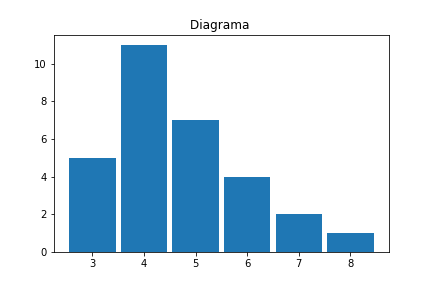
\includegraphics[width=0.7\columnwidth]{diagrama_prueba2} \\ $\left\{ Me : 4.0, \  Mo : \left( [4], \  [11]\right), \  media : 4.67\right\}$ \\$\left\{ P70 : 5.0, \  Q1 : 4.0, \  Q3 : 5.0\right\}$ \\$\left\{ C.V : 0.27, \  desv.tip : 1.27, \  rango : 5, \  var : 1.62\right\}$\\ 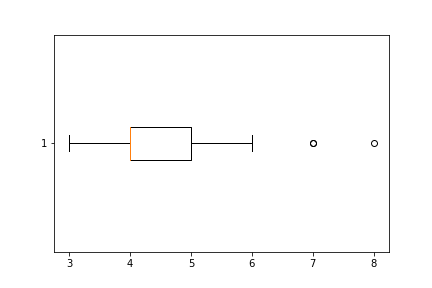
\includegraphics[width=0.7\columnwidth]{caja_prueba2}\end{solution} 

\question Las notas de una clase en el último examen de matemáticas han sido: 3 5 4 5 8 3 5 6 4 5 4 4 3 4 5 6 5 6 4 3 4 4 5 7 4 3 4 4 6 7.

\begin{parts}  
\part[1] Realiza una tabla de frecuencias y un diagrama de barras 
\part[1] Calcular los siguientes parámetros de centralización: media, mediana, moda
\part[1] Calcular los parámetros de posición P90, Q1, Q3
\part[1] Calcular los siguientes parámetros de dispersión: Varianza, Desviación típica y coeficiente de variación 
\part[1]Realiza un diagrama de caja y bigote. 
\part[1] Si se selecciona a una persona al azar de las que están aprobadas, ¿qué probabilidad hay de que al menos haya obtenido notable?  
\end{parts} 
\begin{solution} $\begin{tabular}{rrrrrrr}
\hline
   $x_i$ &   $f_i$ &   $F_i$ &      $\%_i$ &    $\%A_i$ &   $x_if_i$ &   $x^2_if_i$ \\
\hline
       3 &       5 &       5 &  16.6667  &  16.6667 &         15 &           45 \\
       4 &      11 &      16 &  36.6667  &  53.3333 &         44 &          176 \\
       5 &       7 &      23 &  23.3333  &  76.6667 &         35 &          175 \\
       6 &       4 &      27 &  13.3333  &  90      &         24 &          144 \\
       7 &       2 &      29 &   6.66667 &  96.6667 &         14 &           98 \\
       8 &       1 &      30 &   3.33333 & 100      &          8 &           64 \\
     nan &      30 &     nan & 100       & nan      &        140 &          702 \\
\hline
\end{tabular}$\\ 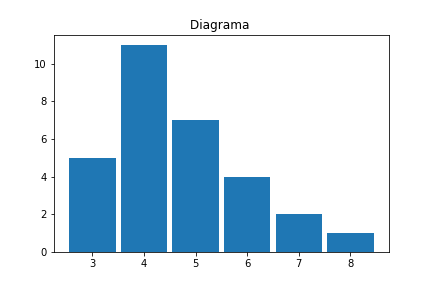
\includegraphics[width=0.7\columnwidth]{diagrama_prueba2} \\ $\left\{ Me : 4.0, \  Mo : \left( [4], \  [11]\right), \  media : 4.67\right\}$ \\$\left\{ P70 : 5.0, \  Q1 : 4.0, \  Q3 : 5.0\right\}$ \\$\left\{ C.V : 0.27, \  desv.tip : 1.27, \  rango : 5, \  var : 1.62\right\}$\\ 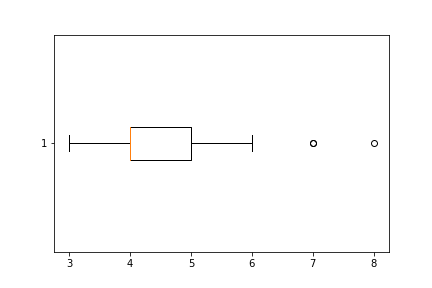
\includegraphics[width=0.7\columnwidth]{caja_prueba2}\end{solution} 

% \question[2] Se lanzan al aire tres monedas. Determinar la probabilidad de que se obtenga al menos dos cruces

\question[2] Un test consta de cuatro preguntas con dos posibles respuestas cada una, una cierta y otra falsa. Si un
estudiante contesta al azar, calcular la probabilidad de acertar al menos dos preguntas

\addpoints

\end{questions}

\end{document}
%\grid
